\documentclass[12pt]{amsart}
\usepackage{amsthm}
\usepackage{hyperref}
\usepackage{a4wide}
\usepackage{array, xcolor}
\usepackage{amsfonts}
\usepackage{amsmath}
\usepackage{mathtools}
\usepackage{amssymb}
\usepackage{graphicx}
\usepackage{float}
\usepackage{accents}
\usepackage{verbatim}
\newtheorem{proposition}{Proposition}%[section]
\newtheorem{lemma}[proposition]{Lemma}
\newtheorem{corollary}[proposition]{Corollary}
\newtheorem{theorem}[proposition]{Theorem}
\usepackage{tikz}
\usepackage{tikz-cd}
\usetikzlibrary{matrix}

\theoremstyle{definition}
\newtheorem{definition}[proposition]{Definition}
\newtheorem{remark}[proposition]{Remark}
\newtheorem*{remark*}{Remark}

\def\RR{{\mathbb R}}
\def\Rn{{\mathbb R^n}}
\def\oRn{{\overline{\mathbb R ^ n}}}
\def\ZZ{{\mathbb Z}}
\def\NN{{\mathbb N}}
\def\CC{{\mathbb C}}
\def\HH{{\mathbb{H}}}
\def\DD{{\mathbb{D}}}
\def\g{{\gamma}}
\def\G{{\Gamma}}


\DeclareMathOperator{\tr}{Tr}
\DeclareMathOperator{\A}{A}
\DeclareMathOperator{\B}{B}
\DeclareMathOperator{\D}{D}
\DeclareMathOperator{\PP}{P}
\DeclareMathOperator{\res}{Res}
\DeclareMathOperator{\psl}{PSL_2(\mathbb{R})}
\DeclareMathOperator{\pslf}{PSL_n(\mathbb{F})}

\DeclareMathOperator{\F}{\Phi}
\DeclareMathOperator{\area}{Area}
\DeclareMathOperator{\vol}{Vol}
\DeclareMathOperator{\rank}{rank}
\DeclareMathOperator{\spec}{Spec}
\DeclareMathOperator{\End}{End}


\newcommand{\cl}{\operatorname{Cl}}
\newcommand{\li}{\operatorname{Li}}
\newcommand{\gl}{\operatorname{GL}}
\newcommand{\slinear}{\operatorname{SL}}
\newcommand{\diam}{\operatorname{Diam}}
\newcommand{\so}{\operatorname{SO}}
\newcommand{\spin}{\operatorname{Spin}}
\newcommand{\supp}{\operatorname{supp}}
\newcommand{\im}{\operatorname{Im}}
\newcommand{\id}{\operatorname{id}}
\newcommand{\Id}{\operatorname{Id}}
\newcommand{\aut}{\operatorname{Aut}}
\newcommand{\deck}{\operatorname{Deck}}

%\setlength\parindent{0pt}
%\setlength\parskip{3pt}


\begin{document}
\title[Spin structures and class functions on Fuchsian groups]{Spin structures and class functions on Fuchsian groups}
\author{Rare\c s Stan}
\address{Institute of Mathematics of the Romanian Academy\\ 
Bucharest\\ 
Romania}
\email{rares.stan@imar.ro}

\begin{abstract}
We study a class function induced by the spin structure on complete oriented hyperbolic surfaces. Two apparently different definitions are presented and in the end we show the equivalence of these definitions.
\end{abstract}

\date{\today}
\maketitle

\section{Introduction}
Consider $\G\setminus \HH$ an oriented complete hyperbolic surface of finite area, where $\G\subset \psl$ is a Fuchsian group without elliptic ellements and $\HH$ is the hyperbolic plane. These surfaces always admit spin structures, since their Euler class is even. The purpose of this paper is to study a class function $\varepsilon: \G \longrightarrow \{ \pm 1 \}$, namely a function which is constant along conjugacy classes, induced by a spin structure. The class function in question first appeared in \cite{dhockerPhong}, where D'Hocker and Phong prove that determinants of connection laplacians on spinors on Riemann surfaces can be computed in terms of the Selberg zeta function at half integer points. It also appears in \cite{SarnckDeterminantsOfLaplacians}, where a similar statement is proven for Dirac operators; note  that the class function seems to be inadvertently considered as a group morphism, which it is not, as we shall see below. We shall see below that this is not the case. The same functions also appears in \cite{BolteStiepanSelbergForDirac}, a paper where a Seleberg trace formula is proved for Dirac operators on compact hyperbolic surfaces. Later, in \cite{rares}, the author obtains an asymptotic for the Selberg zeta function at some parts of the boundary of the Teichm\" uler space. Here $\varepsilon$ plays a crucial role as the same result cannot hold true for the Laplace operator.

Spin structures are well understood in a very wide generality. The novelty in this paper is the rigorous presentation of the class function $\varepsilon$, since it is only briefly introduced in all the above mentioned papers. We start with a brief introduction of spin structures on general manifolds (for more details see, e.g. \cite{carteMoroianuSpinori, hitchin, lawsonMichelsohn}) and afterwards restrict ourselves to oriented complete hyperbolic surfaces. These surfaces can be regarded as $\G\setminus \HH$, where $\HH$ is the hyperbolic plane and $\G$ is a discrete subgroup of $\psl$. For clarity, we will interpret the spinor bundle as the group of $2\times2$ matrices of determinant $1$, $\slinear_2(\RR)$. We give two different definitions for the class functions, one in term of algebraic extensions, and a more geometric one, which for hyperbolic elements is exactly the holonomy along the associated closed geodesics. We prove, in Theorem \ref{teoremEgalitateDefinitii}, that these two definitions are equivalent.

\subsection*{Acknowledgements} 
I would like to thank Sergiu Moroianu for his advise during the preparation of this paper. I am also grateful to Léo Bénard, Laura Monk, Bernd Ammann and Julian Seipel for their valuable conversations and input.

\subsection*{Funding}
The author was partially supported from the project PNRR–III-C9–2023–I8.

\section{Spin structures on Riemannian manifolds}
For a positive integer $n$ consider the vector space $\RR^n$ endowed with the standard scalar product. The \emph{Clifford algebra} $\cl_n$ is the quotient of the tensor algebra $T(\RR^n):=\oplus_{j=0}^{\infty} (\RR^n)^{\otimes j}$ by the \emph{Clifford ideal}, that is the ideal generated by all the tensors of the form $v\otimes v + \|v \|^2$. The \emph{spin group} $\spin(n)$ is the group of even products of unit vectors. It is a connected, two-sheeted covering for the special orthogonal group $\so(n)$ (the universal cover of $\so(n)$ for $n\geq 3$). 
Let us compute it now. In terms of the standard basis $\{e_1,e_2 \}$ of $\RR^2$ it is easy to see that:
\[
\cl_2 = \RR \oplus e_1\RR \oplus e_2\RR \oplus e_1e_2\RR,
\]
which is isomorphic with the field of quaternions. The unit vectors in $\cl_2$ have the form $v=ae_1+be_2$, with $a^2+b^2=1$. Therefore $\spin(2)$ consists of all the elements of the form:
\begin{align*}
vw
&=
(ae_1+b_e2)(ce_1+d_e2)
=-(ac+bd) + (ad-bc)e_1e_2 \\
&= a' + b' e_1e_2,
\end{align*}
where $(a')^2+(b')^2=1$.
\begin{remark}\label{spinRotationsIsomorphism}
It follows that $\spin(2)$ is isomorphic to the group of rotation matrices: 
\begin{align*}
\left\lbrace
R(\theta):=
\begin{bmatrix}
\cos \theta & -\sin \theta \\
\sin \theta & \cos \theta
\end{bmatrix}
:
\theta \in [0,2\pi]
\right\rbrace.
\end{align*}
\end{remark}

When $n = 2k$, the complexified Clifford algebra $\cl_n \otimes \RR$ is isomorphic to the algebra of complex matrices of order $2^{n/2}$. To see this isomorphism take $\{ e_1,..., e_{2k} \}$ the standard basis in $\RR^n$ and consider $W$ the vector space generated by $\{ 2^{-1/2}(e_1 -ie_2), ..., 2^{-1/2}(e_{2k-1} - ie_{2k}) \}$. Clearly, the representation:
\[
cl(v):=\frac{1}{\sqrt{2}}(v-Jv)\wedge(\cdot) - \frac{1}{\sqrt{2}}(v+iJv)\lrcorner(\cdot),
\]
where $J$ is the standard almost complex structure, acts on $\Sigma_n:=\wedge^*W$ and can be extended to the tensor algebra $T(\CC^n)$. A simple computation leads us to the conclusion that $cl$ descends to the complexified Clifford algebra:
\begin{align*}
cl : \cl_n\otimes_{\RR}\CC \longrightarrow \End_{\CC} (\Sigma_n) \simeq M(2^k ,\CC).
\end{align*}

Consider now $M$ an oriented Riemannian manifold and $P_{\so(n)}M$ the oriented frame bundle. A \emph{spin structure} on $M$ is a $\spin(n)$ principal bundle $P_{\spin(n)}M$ together with two covering maps $\pi_1$, $\pi_2$ which makes the following diagram:
\begin{equation}\label{spinStructureDiagram}
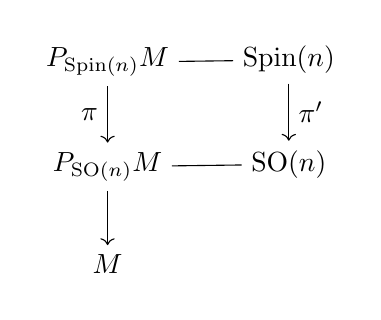
\begin{tikzpicture}[baseline=(current  bounding  box.center)]
  \matrix (m) [matrix of math nodes,row sep=2em,column sep=2em,minimum width=2em]
  {
      P_{\text{Spin}(n)} M & \text{Spin}(n) \\
        P_{\text{SO}(n)} M & \text{SO}(n) \\
	    M & {} \\  
  };
  \path
    (m-1-1) edge node [ above] {} (m-1-2)
    (m-2-1) edge node [below] {} (m-2-2);
    
    
  \path[->] 
  	(m-1-1) edge node [left]{$\pi$} (m-2-1)
  	(m-1-2) edge node [right] {$\pi'$} (m-2-2)
  	(m-2-1) edge node [left] {} (m-3-1);
\end{tikzpicture}
\end{equation}
satisfy $\pi(xs) = \pi(x) \pi'(s)$ for any $s\in \spin(n)$ and $x \in P_{\spin(n)} M$.

\section{Spin structures on hyperbolic surfaces}
We shall focus on oriented complete hyperbolic surfaces form now on. These are smooth oriented surfaces of constant curvature $-1$. From Hadamard's theorem we know that there exists a unique simply connected, complete, hyperbolic surface up to isometry. 
\subsection{The hyperbolic plane}
One can use many models of this unique surface, but for the purpose of this paper we will restrict ourselves to the hyperbolic plane. Recall that the hyperbolic plane is the upper half plane endowed with a metric of constant curvature $-1$:
\[
\HH := \left( \{ (x,y)\in \RR^2 : \ y>0 \}, \ g=\frac{dx^2+ dy^2}{y^2} \right).
\]
We show that $\HH$ admits a spin structure and, moreover, the bundle $P_{\spin(2)}\HH$ can be identified with $\slinear_2(\RR)$ as $\spin(2)$ principal bundles. The orientation preserving isometries of $\HH$ are given by the group $\psl := \slinear_2(\RR) / \{\pm 1 \}$ with the action:
\begin{align*}
\g z = \frac{az+b}{cz+d}, && \g= \begin{bmatrix} a & b \\
                                                                                  c & d   \end{bmatrix} \in \slinear_2(\RR),
\end{align*}
for any $z = x+iy\in \CC \simeq \RR^2$ with $\Im z >0$. Through direct computations one can see that a given orientation preserving isometry can be completely determined by the way it moves a point and a vector at that point. The mapping:
\begin{align}\label{pslTangenSpaceIdentification}
\g \mapsto \left( \g i, \left\{ \g_{*,i} \left( \frac{\partial}{\partial x} \right) ,\g_{*,i} \left( \frac{\partial}{\partial y} \right) \right\} \right).
\end{align} is well defined for products of isometries as well. Hence the oriented orthogonal frame bundle $P_{\so(2)}\HH$ and $\psl$ can be identified as $\so(2)$ principal bundles. Moreover, the action induced by orientation preserving isometries to the orthonormal frame bundle:
\begin{align*}
\g_*:P_{\so (2)}\HH\longrightarrow P_{\so (2)}\HH, && 
\g_*\left(z, \{ v_1, v_2 \} \right) = \left( \g z, \{ \g_{*,z}v_1, \g_{*,z}v_2 \} \right),
\end{align*}
is transformed by the previous mapping into the left multiplication:
\begin{align*}
\g:\psl \longrightarrow \psl, && 
\g(\eta) = \g \eta.
\end{align*}

\begin{proposition}\label{spinStructureForH}
$\slinear_2(\RR)$ is a $\spin(2)$ principal bundle over $\HH$. Moreover, with the projections $\pi': \spin(2)\simeq \{R(\theta):\theta\in [0,2\pi] \} \longrightarrow \so(2)\simeq \{R(\theta):\theta\in [0,2\pi] \}$ and $\pi: \slinear_2(\RR) \longrightarrow \psl$ defined by:
\begin{align*}
\pi'(R(\theta))
&= R(-2\theta);\\
\pi\left(
\begin{bmatrix}
a & b\\
c & d
\end{bmatrix}
\right)
&=
\left(
z \mapsto \frac{az+b}{cz + d},
\right),
\end{align*}
the following diagram is commutative:
\begin{equation}\label{spinStructureHDiagram}
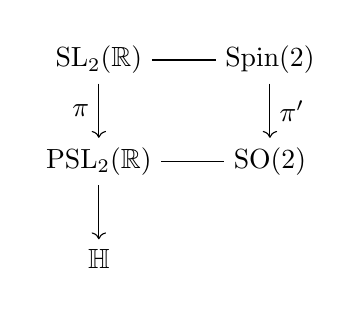
\begin{tikzpicture}[baseline=(current  bounding  box.center)]
  \matrix (m) [matrix of math nodes,row sep=2em,column sep=2em,minimum width=2em]
  {
      \slinear_2(\RR)& \spin(2) \\
      \psl & \so(2) \\
	    \HH & {} \\  
  };
  \path
    (m-1-1) edge node [ above] {} (m-1-2)
    (m-2-1)	edge node [below] {} (m-2-2);
    
    
  \path[->] 
  	(m-1-1) edge node [left]{$\pi$} (m-2-1)
  	(m-1-2)	edge node [right] {$\pi'$} (m-2-2)
  	(m-2-1) edge node [left] {} (m-3-1);
\end{tikzpicture}
\end{equation}
and hence $\HH$ admits a spin structure with $P_{\spin(2)}\HH \simeq \slinear_2(\RR)$.
\end{proposition}
\begin{proof}
We start with the first part. If $A\in \slinear_2(\RR)$ and $z\in \HH$ then by $Az$ we naturally understand:
\begin{align*}
A = 
\begin{bmatrix} a & b \\ c & d   \end{bmatrix};
&&
Az := \frac{az+b}{cz +d}.
\end{align*}
By the Iwasawa decomposition theorem, every $A\in \slinear_2(\RR)$ can be uniquely written as:
\begin{align*}
A &= 
\begin{bmatrix} 
1 & \Re (Ai) \\ 
0 &   1
\end{bmatrix}
\begin{bmatrix} 
\sqrt{\Im(Ai)} & 0 \\ 
0 &   \frac{1}{\sqrt{\Im(Ai)}}
\end{bmatrix}
\begin{bmatrix} 
\cos \theta & -\sin \theta \\ 
\sin \theta &   \cos \theta 
\end{bmatrix}
\\
&
=: T(\Re(Ai))D\left(\sqrt{\Im(Ai)}\right)R(\theta)
,
\end{align*}
for some $\theta \in [0,2\pi]$. Thus, the fibre over $\HH$ at a given point $z=Ai$ is given by all the matrices that map $i$ into $z$, namely:
\begin{align*}
(\slinear_2(\RR))_z = 
\left\lbrace
T(\Re z)D\left( \sqrt{\Im z}\right) R(\theta)
:
\theta \in [0,2\pi]
\right\rbrace.
\end{align*}
Clearly, the group $\left\lbrace
R(\theta)
:
\theta \in [0,2\pi]
\right\rbrace$ acts freely and transitively on the fibres $(\slinear_2(\RR))_z$ and thus $\slinear_2(\RR)$ is a principal bundle with group $\spin(2)$ over $\HH$. 

For the second part, notice that the isometries $(z\mapsto T(\Im z))$ and $(z\mapsto D(\sqrt{\Re z)})$ act as the identity on the oriented frames. Therefore it is enough to check that the diagram $(\ref{spinStructureHDiagram})$ is commutative only for matrices in the fibre over $i\in \HH$:
\begin{align*}
R(\theta)_{*,i}\left( \frac{\partial}{\partial x} \right)
&=
\left. \frac{\partial}{\partial x} \right|_{x+iy=i} \left( \frac{x\cos \theta + iy\cos \theta - \sin \theta}{x\sin \theta + iy\sin \theta + \cos \theta} \right) = \cos 2\theta - i \sin 2\theta
\simeq 
\begin{bmatrix}
\cos 2\theta \\
-\sin 2\theta
\end{bmatrix}
;\\
R(\theta)_{*,i}\left( \frac{\partial}{\partial y} \right)
&=
\left. \frac{\partial}{\partial y} \right|_{x+iy=i} \left( \frac{x\cos \theta + iy\cos \theta - \sin \theta}{x\sin \theta + iy\sin \theta + \cos \theta} \right) = i(\cos 2\theta - i \sin 2\theta)
\simeq 
\begin{bmatrix}
\sin 2\theta \\
\cos 2\theta
\end{bmatrix}
.
\end{align*}
This leads to:
\begin{align*}
R(\theta)_{*,i}:T_i\HH \longrightarrow T_i\HH
&&
R(\theta)_{*,i}\simeq
\begin{bmatrix}
\cos 2\theta & \sin 2\theta \\
-\sin 2\theta & \cos 2\theta
\end{bmatrix},
\end{align*}
and thus $\pi(R(\theta))=R(-2\theta)=\pi(I_2)\pi'(R(\theta))$.
\end{proof}

\begin{proposition}\label{oneSpinStructure}
There exists only one spin structure over $\HH$ up to isomorphism.
\end{proposition}
\begin{proof}
Consider a spin structure over $\HH$, namely a $\spin(2)$ principal bundle $P$ covering $P_{\so(2)}\HH$ making diagram $(\ref{spinStructureDiagram})$ commute. Our aim is to find an isomorphism $\phi$ such that the following diagram:
\begin{equation}\label{diagramPiPhi}
\begin{tikzcd}
P \arrow{dr}[swap]{\pi} \arrow[dashed]{rr}{\phi} && \slinear_2(\RR) \arrow{dl}{\pi} \\
& P_{\so(2)}\HH
\end{tikzcd}
\end{equation}
commutes as well. Since $\HH$ is simply connected $P_{\so(2)}\HH$ is trivial and can be identified with $\HH\times \so(2)$. Take $s(z):=\left( z,\begin{bmatrix}
1 & 0 \\
0 & 1
\end{bmatrix} \right)$ the standard global section and lift it to $P$:
\begin{equation*}
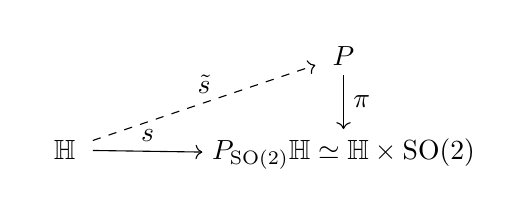
\begin{tikzpicture}[baseline=(current  bounding  box.center)]
  \matrix (m) [matrix of math nodes,row sep=2em,column sep=4em,minimum width=2em]
  {
      {} & P \\
      \HH & P_{\so(2)}\HH \simeq \HH\times \so(2) \\
  };
  \path[->]
    (m-2-1) edge node [ above] {$s$} (m-2-2)
    (m-1-2) edge node [right] {$\pi$} (m-2-2)
    (m-2-1)	edge [dashed] node [above] {$\tilde{s}$} (m-1-2);
\end{tikzpicture}
\end{equation*}
Note that $\phi : P \longrightarrow \slinear_2(\RR)$ must be compatible with the right $\spin(2)$ right multiplication, hence it is enough to define it on $\tilde{s}$:
\begin{align*}
\phi(\tilde{s}(z)) := T(\Re(z))D(\sqrt{\Im(z)}).
\end{align*}
Every $p\in P$ can be uniquely written as $\tilde{s} R$, for $R\in \spin(2)$, hence, we have that:
\begin{align*}
\pi(p) = \pi(\tilde{s}R) = s\pi'(R) = \pi\left( T(\Re(z))D(\sqrt{\Im(z)})\right) \pi'(R),
\end{align*}
which concludes the proof.
\end{proof}

\subsection{Hyperbolic surfaces}
Consider $M = \G \setminus \HH$ a hyperbolic surface of finite area, where $\G \subset \psl$. As we mentioned earlier, the group $\G$ acts on $\psl$ through the left multiplication. However, we claim that the principal bundle $P_{\so_2(\RR)}M \simeq \G \setminus \psl$ has no additional algebraic structure. Indeed, since $\G$ is discrete, the map $\alpha \mapsto \alpha\g \alpha^{-1}$, for $\g \in \G$ and $\alpha\in \psl$, is constant. Thus $\psl$ has no trivial discrete normal subgroup. Moreover, Dickson proved in \cite{dickson} that $\pslf$ has no normal subgroups, where $\mathbb{F}$ is an infinite field and $n\geq2$. 

If we denote by $\tilde{\G}:= \pi^{-1}(\G)$ then we have the following exact sequence:
\begin{align}\label{exactSequence}
 1 \longrightarrow \{ \pm 1 \} \longrightarrow \tilde{\G} \longrightarrow \G \longrightarrow 1.
\end{align}

\begin{proposition}
The spin structures on $M$ are in one-to-one correspondence with splitting morphisms (of the exact sequence $(\ref{exactSequence})$) $\rho : \G \longrightarrow \tilde{\G}$ with $\pi\circ \rho = \Id_{\G}$.
\end{proposition}
\begin{proof}
We start with the easier part. Consider $\rho : \G \longrightarrow \tilde{\G}$ a splitting. 
Clearly, from Proposition \ref{spinStructureForH}, the quotient $\rho(\G)\setminus \slinear_2(\RR)$ is a two-sheeted cover of $\G \setminus \psl$. Moreover the diagram:
\begin{equation*}
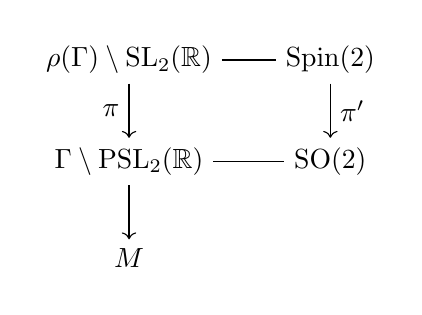
\begin{tikzpicture}[baseline=(current  bounding  box.center)]
  \matrix (m) [matrix of math nodes,row sep=2em,column sep=2em,minimum width=2em]
  {
      \rho(\G)\setminus \slinear_2(\RR)& \spin(2) \\
      \G\setminus\psl & \so(2) \\
	    M & {} \\  
  };
  \path
    (m-1-1) edge node [ above] {} (m-1-2)
    (m-2-1)	edge node [below] {} (m-2-2);
    
    
  \path[->] 
  	(m-1-1) edge node [left]{$\pi$} (m-2-1)
  	(m-1-2)	edge node [right] {$\pi'$} (m-2-2)
  	(m-2-1) edge node [left] {} (m-3-1);
\end{tikzpicture}
\end{equation*}
is commutative, since:
\begin{align*}
\pi([AR(\theta)])=[\pi(AR(\theta)]=[\pi(A)\pi'(R(\theta))]=\pi([A])R(-2\theta).
\end{align*}

Now let us consider a spin structure on $\G \setminus \HH$ and denote by $p:\HH \longrightarrow \G\setminus \HH$ the canonical projection. Since the group $\G$ acts on the frame bundle over $\HH$, we get that the pull-back bundle $p^*(P_{\so(2)}(\G\setminus \HH))$ is isomorphic to $P_{\so(2)} \HH$. We consider the following pull-back:
\begin{equation}\label{diagramPullBack}
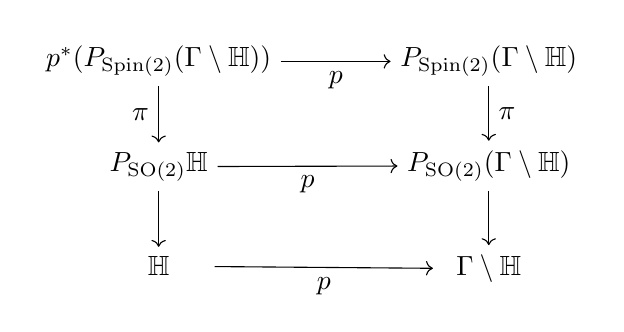
\begin{tikzpicture}[baseline=(current  bounding  box.center)]
  \matrix (m) [matrix of math nodes,row sep=2em,column sep=4em,minimum width=4em]
  {
      p^*(P_{\spin(2)}(\G\setminus \HH)) & P_{\spin(2)}(\G\setminus \HH) \\
      P_{\so(2)} \HH & P_{\so(2)}(\G\setminus \HH) \\
	    \HH & \G\setminus \HH \\  
  };
  \path[->]
    (m-1-1) edge node [below] {$p$} (m-1-2)
    (m-2-1)	edge node [below] {$p$} (m-2-2)
    (m-3-1) edge node [below] {$p$} (m-3-2);
    
  \path[->] 
  	(m-1-1) edge node [left]{$\pi$} (m-2-1)
  	(m-1-2)	edge node [right] {$\pi$} (m-2-2)
  	(m-2-1) edge node [left] {} (m-3-1)
  	(m-2-2) edge node [right] {} (m-3-2);
\end{tikzpicture}
\end{equation}
Clearly $p^*(P_{\spin(2)}(\G\setminus \HH))$ defines a spin structure, hence, from Proposition $\ref{oneSpinStructure}$, there exists an isomorphism $\phi:p^*(P_{\spin(2)}(\G\setminus \HH)) \longrightarrow \slinear_2(\RR)$. Moreover, there exists a canonical action $\rho'$ of $\G$ on the bundle $p^*(P_{\spin(2)}(\G\setminus \HH))$. For $\g\in \G$, $\rho'(\g)$ moves a base point $z$ to $\g z$ and acts as the identity on the respective fibres. Therefore, we can define the function $\rho$ on $\G$ as follows: 
\begin{align*}
\rho(\g) = \phi \circ\rho'(\g)\circ \phi^{-1}.
\end{align*}
In this way, $\rho(\g)$ is a $\spin(2)$ principal bundle isomorphism. Our aim is to show that, in fact, $\rho(\g)$ is actually a matrix that lies in $\tilde{\G}$. For $q\in \slinear_2(\RR)$, using diagrams $(\ref{diagramPiPhi})$, $(\ref{diagramPullBack})$ and again $(\ref{diagramPiPhi})$, we have that:
\begin{align*}
\pi(\rho(\g)q)
&=
\pi(\phi \circ \rho'(\g) \circ \phi^{-1}(q))
=
\pi(\rho'(\g) \circ \phi^{-1}(q))
=
\g\pi(\phi^{-1}(q))
=
\g\pi(q).
\end{align*}
Thus $\rho(\g)q\in \{ \tilde{\g}_1 q, \tilde{\g}_2 q \}$ for any $q\in \slinear_2(\RR)$, where $\tilde{\g}_1$ and $\tilde{\g}_2$ are the two lifts of $\g\in \G \subset \psl$ to $\slinear_2(\RR)$. It follows that the map $q \mapsto \left( \rho(\g)(q) \right) q^{-1}$ is constant and continuous, hence $\rho(\g) \subset \tilde{\G}$. Moreover, $\rho$ is a morphism, since $\rho'$ is an action.
\end{proof}
We have to show that 
Remark that $\rho(\g) \in \pi^{-1}(\g)$ for each $\g \in \G$. For example, if $M$ is compact and there are $2g$ generators for $\G$, then there are in total $2^{2g}$ spin structures. 
The function $\rho$ induces an action from $\G$ to $\slinear_2(\RR)\simeq P_{\spin(2)}\HH$, however, as before, the quotient carries no additional algebraic structure.

\section{Reading the spin structure in a class function}
In this section we talk about a class function induced by the spin structure. It was first introduced by D'Hocker and Phong in \cite{dhockerPhong} and was later used by Sarnack \cite{SarnckDeterminantsOfLaplacians} as well. We start with the definition that appeared in \cite{dhockerPhong}, which is rather algebraic, and then continue with a new, more geometric, interpretation. Finally we prove the equivalence of these two definitions.
\subsection{Algebraic definition}\label{algebraicInterpretation}
We define the class function $\varepsilon: \G \longrightarrow \{ \pm 1 \}$ in the following manner:
\begin{align*}
\varepsilon(\g) := 
\begin{cases}
1 & \tr(\rho(\g)) > 0 ;\\
-1 & \tr(\rho(\g)) < 0.
\end{cases}
\end{align*}
Clearly, from the definition, $\varepsilon$ is a class function, meaning that its value is constant along conjugacy classes. Moreover $\varepsilon(\g^n) = \varepsilon^n(\g)$ for any $n\geq 1$. Obviously there are examples of matrices of positive trace for which the trace of the product is not positive, therefore we cannot expect $\varepsilon$ to be a group morphism. Further notice that manner in which we associate a class function to a spin structure is injective.

\subsection{Geometric definition}\label{geometricInterpretation}
We want to define an apparently different class function $\varepsilon':\G \longrightarrow \{ \pm 1 \}$, however, this definition is not as straight-forward as before.
If $\g\in\G$ is hyperbolic, denote by $\eta$ the unique geodesic in $\HH$ preserved by $\g$ and, for $t\in \RR$, consider the curve $p_{\eta(t)}:= (\eta(t), \{ \dot{\eta}(t), J \dot{\eta}(t)\}) \in P_{\so(2)}\HH$, where $J$ is the standard almost complex structure on $\HH$. Since $\g_*p_{\eta(t)} = \g_*p_{\g\eta(t)}$, the projection of $p$ on $P_{\so(2)}M$ is a closed curve. Take $\tilde{p}$ an arbitrary lift of $p$ to $P_{\spin(2)}\HH$. We define $\varepsilon'$ such that:
\begin{align*}
\rho(\g)\tilde{p}_{\eta(t)} = \varepsilon'(\g)\tilde{p}_{\g\eta(t)}.
\end{align*}
If $\g$ is parabolic then there exists $a\in\psl$ such that $\g=a\tau a^{-1}$, where $\tau$ is the translation by $1$. 
The horocycle $t\mapsto t+i$ is preserved by $\tau$, hence $\mu(t) := a(t+i)$ is a horocycle preserved by $\g$.
It follows that $p_{\mu (t)}:=(\mu(t), \{\dot{\mu}(t),J\dot{\mu}(t) \}) \in P_{\so(2)}\HH$ is $\g$-invariant. Hence, for $\tilde{p}$ a lift of $p$, we can define the class function as in the previous case:
\begin{align*}
\rho(\g)\tilde{p}_{\mu(t)} = \varepsilon'(\g)\tilde{p}_{\g \mu(t)}.
\end{align*}

We remark that if $\g$ is hyperbolic, this definition is exactly the holonomy along the unique geodesic associated to the conjugacy class of $\g$.
\subsection{Equivalence of the two definitions for class functions}

\begin{theorem}\label{teoremEgalitateDefinitii}
Let $\G\setminus \HH$ be a complete hyperbolic surface of finite area, where $\G\subset \psl$. Then, the functions $\varepsilon$ and $\varepsilon'$ defined in \ref{algebraicInterpretation} and \ref{geometricInterpretation} coincide.
\end{theorem}
\begin{proof}
Take $\g\in\G$ a hyperbolic element. Then there exists $l>0$ and $a\in \psl$ such that: 
$\g=a e^l a^{-1}$, where $e^l (z) = e^lz$. Denote by $\eta$ the geodesic in $\HH$ (corresponding to a geodesic of length $l$ on $\G\setminus \HH$) preserved by $\g$. From our previous considerations $\eta(t)=a(ie^t)$ is a parametrization of this geodesic. Moreover, taking the curve $p_{\eta(t)}$ as in section \ref{geometricInterpretation}, we get $p_{\eta(t)}=ae^t\in \psl \simeq P_{\so(2)}\HH$. If we fix $A \in \slinear_2(\RR)$ an arbitrarily lift for $a$, then 
$A\begin{bmatrix}
e^{t/2} & 0 \\
0 & e^{-t/2} \\
\end{bmatrix}$ is a lift of $p$. When $t$ goes from $0$ to $l$ we move along the geodesic once, therefore, from the definition of $\varepsilon'$:
\begin{align*}
\rho(\g) A 
\begin{bmatrix}
1 & 0 \\
0 & 1 \\
\end{bmatrix}  &= \varepsilon'(\g) 
A
\begin{bmatrix}
e^{l/2} & 0 \\
0 & e^{-l/2} \\
\end{bmatrix}.
\end{align*}
Thus $\tr (\rho(\g)\varepsilon'(\g))>0$, and hence, from the definition in section \ref{algebraicInterpretation}, $\varepsilon(\g)=\varepsilon'(\g)$.

Let us now consider the case when $\g\in \G$ is a parabolic element. There exists $a\in\psl$ such that $\g=a\tau_1 a^{-1}$ where $\tau_s z := z+s$. Then, the horocycle $\mu(t)=a(t+i)$ is preserved by $\g$.
Moreover, notice that the frame $\left( \tau_t(i), \left\lbrace \frac{\partial}{\partial x}, \frac{\partial}{\partial y} \right\rbrace\right) \in P_{\so(2)}\HH$ corresponds to $\tau_t \in \psl$. It follows that $p_{\mu(t)}=a\tau_t$, via the mapping $(\ref{pslTangenSpaceIdentification})$. As before, if we consider $A\in\slinear_2(\RR)$ an arbitrary lift of $a$, then
$A\begin{bmatrix}
1 & t \\
0 & 1 \\
\end{bmatrix}$
is a lift of $p$ and hence:
\begin{align*}
\rho(\g) A 
\begin{bmatrix}
1 & 0 \\
0 & 1 \\
\end{bmatrix}  &= \varepsilon'(\g) 
A
\begin{bmatrix}
1 & 1 \\
0 & 1 \\
\end{bmatrix}.
\end{align*}
The conclusion follows as in the previous case.
\end{proof}

\begin{thebibliography}{99}

\bibitem{BolteStiepanSelbergForDirac}
J.~Bolte, H.~M.~Stiepan, \emph{The Selberg trace formula for Dirac operators}, J. Math. Phys. \textbf{47} (2006), no. 11.

\bibitem{carteMoroianuSpinori}
J.~P.~Bourguignon, O.~Hijazi, J.~L.~Milhorat, A.~Moroianu, S.~Moroianu, \emph{A Spinorial Approach to Riemannian and Conformal Geometry}, EMS Monographs in Mathematics. European Mathematical Society (EMS), Zürich, 2015.

\bibitem{dhockerPhong}
E.~D'Hoker, D.~H.~Phong, \emph{On determinants of Laplacians on Riemann surfaces}, Comm. Math. Phys. \textbf{104} (1986), no. 4, 537--545.

\bibitem{dickson}
L.~E.~Dickson, \emph{Theory of linear groups in an arbitrary field}, Trans. Amer. Math. Soc. \textbf{2} (1901), 363–-394.

\bibitem{hitchin}
N.~Hitchin, \emph{Harmonic Spinors}, Advances in Mathematics \textbf{14} (1974), no. 1, 1--55.

\bibitem{lawsonMichelsohn}
H.~B.~Lawson, M.~L.~Michelsohn, \emph{Spin Geometry}, Princeton University Press, (PMS-38), 1989.

\bibitem{SarnckDeterminantsOfLaplacians}
P.~Sarnak, \emph{Determinants of Laplacians},  Comm. Math. Phys. \textbf{110} (1987), no. 1, 113--120.


\bibitem{rares}
R.~Stan, \emph{The Selberg trace formula for spin Dirac operators on degenerating hyperbolic surfaces}, \url{https://arxiv.org/abs/2212.11793}.


\end{thebibliography}
 

\end{document}
